\chapter{System functionality}
\section{Introduction}
This chapter describes the system architecture, the plan, and the test result. First, the chapter begins with the system architecture which consists of the system functionality and main functions. The system functionality describes the components of the system and the overall structure of the system. The main function section describes all the functions in the system. Lastly, the test plan and the results explain the processes and procedures used for testing the system.
\section{4.2 System architecture}

\begin{figure}[!h]
    \centering
    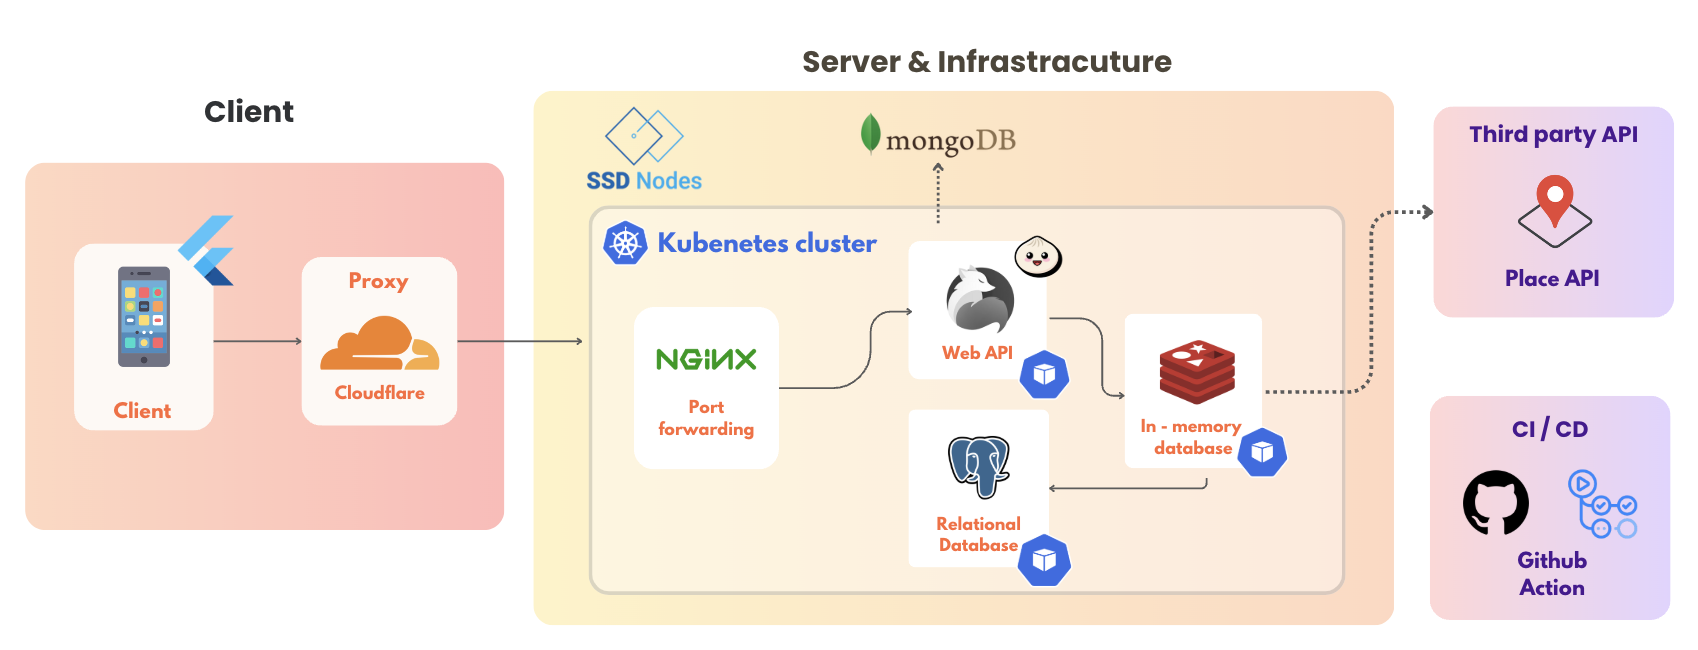
\includegraphics[width=1\linewidth]{chapter4/sysarch.png}
    \caption{System architecture}
    \label{Figure 4-1. System architecture}
\end{figure}
The PlanADay software architecture employs a client-server model, with the frontend handling user interaction through screens and forms, and the backend managing core logic, API integrations, and database operations. The frontend allows users to create plans, customize them, or authenticate via registration and login, sending input to the backend for processing. The backend retrieves data from external APIs like Google Places, caches it for efficient reuse, verifies user credentials using token-based authentication, and stores user data securely. This architecture prioritizes separation of concerns, efficiency through caching, and security, ensuring a scalable and user-friendly system for generating and customizing plans.

\section{4.3 Test Plan}
\begin{figure}[!h]
	\centering
	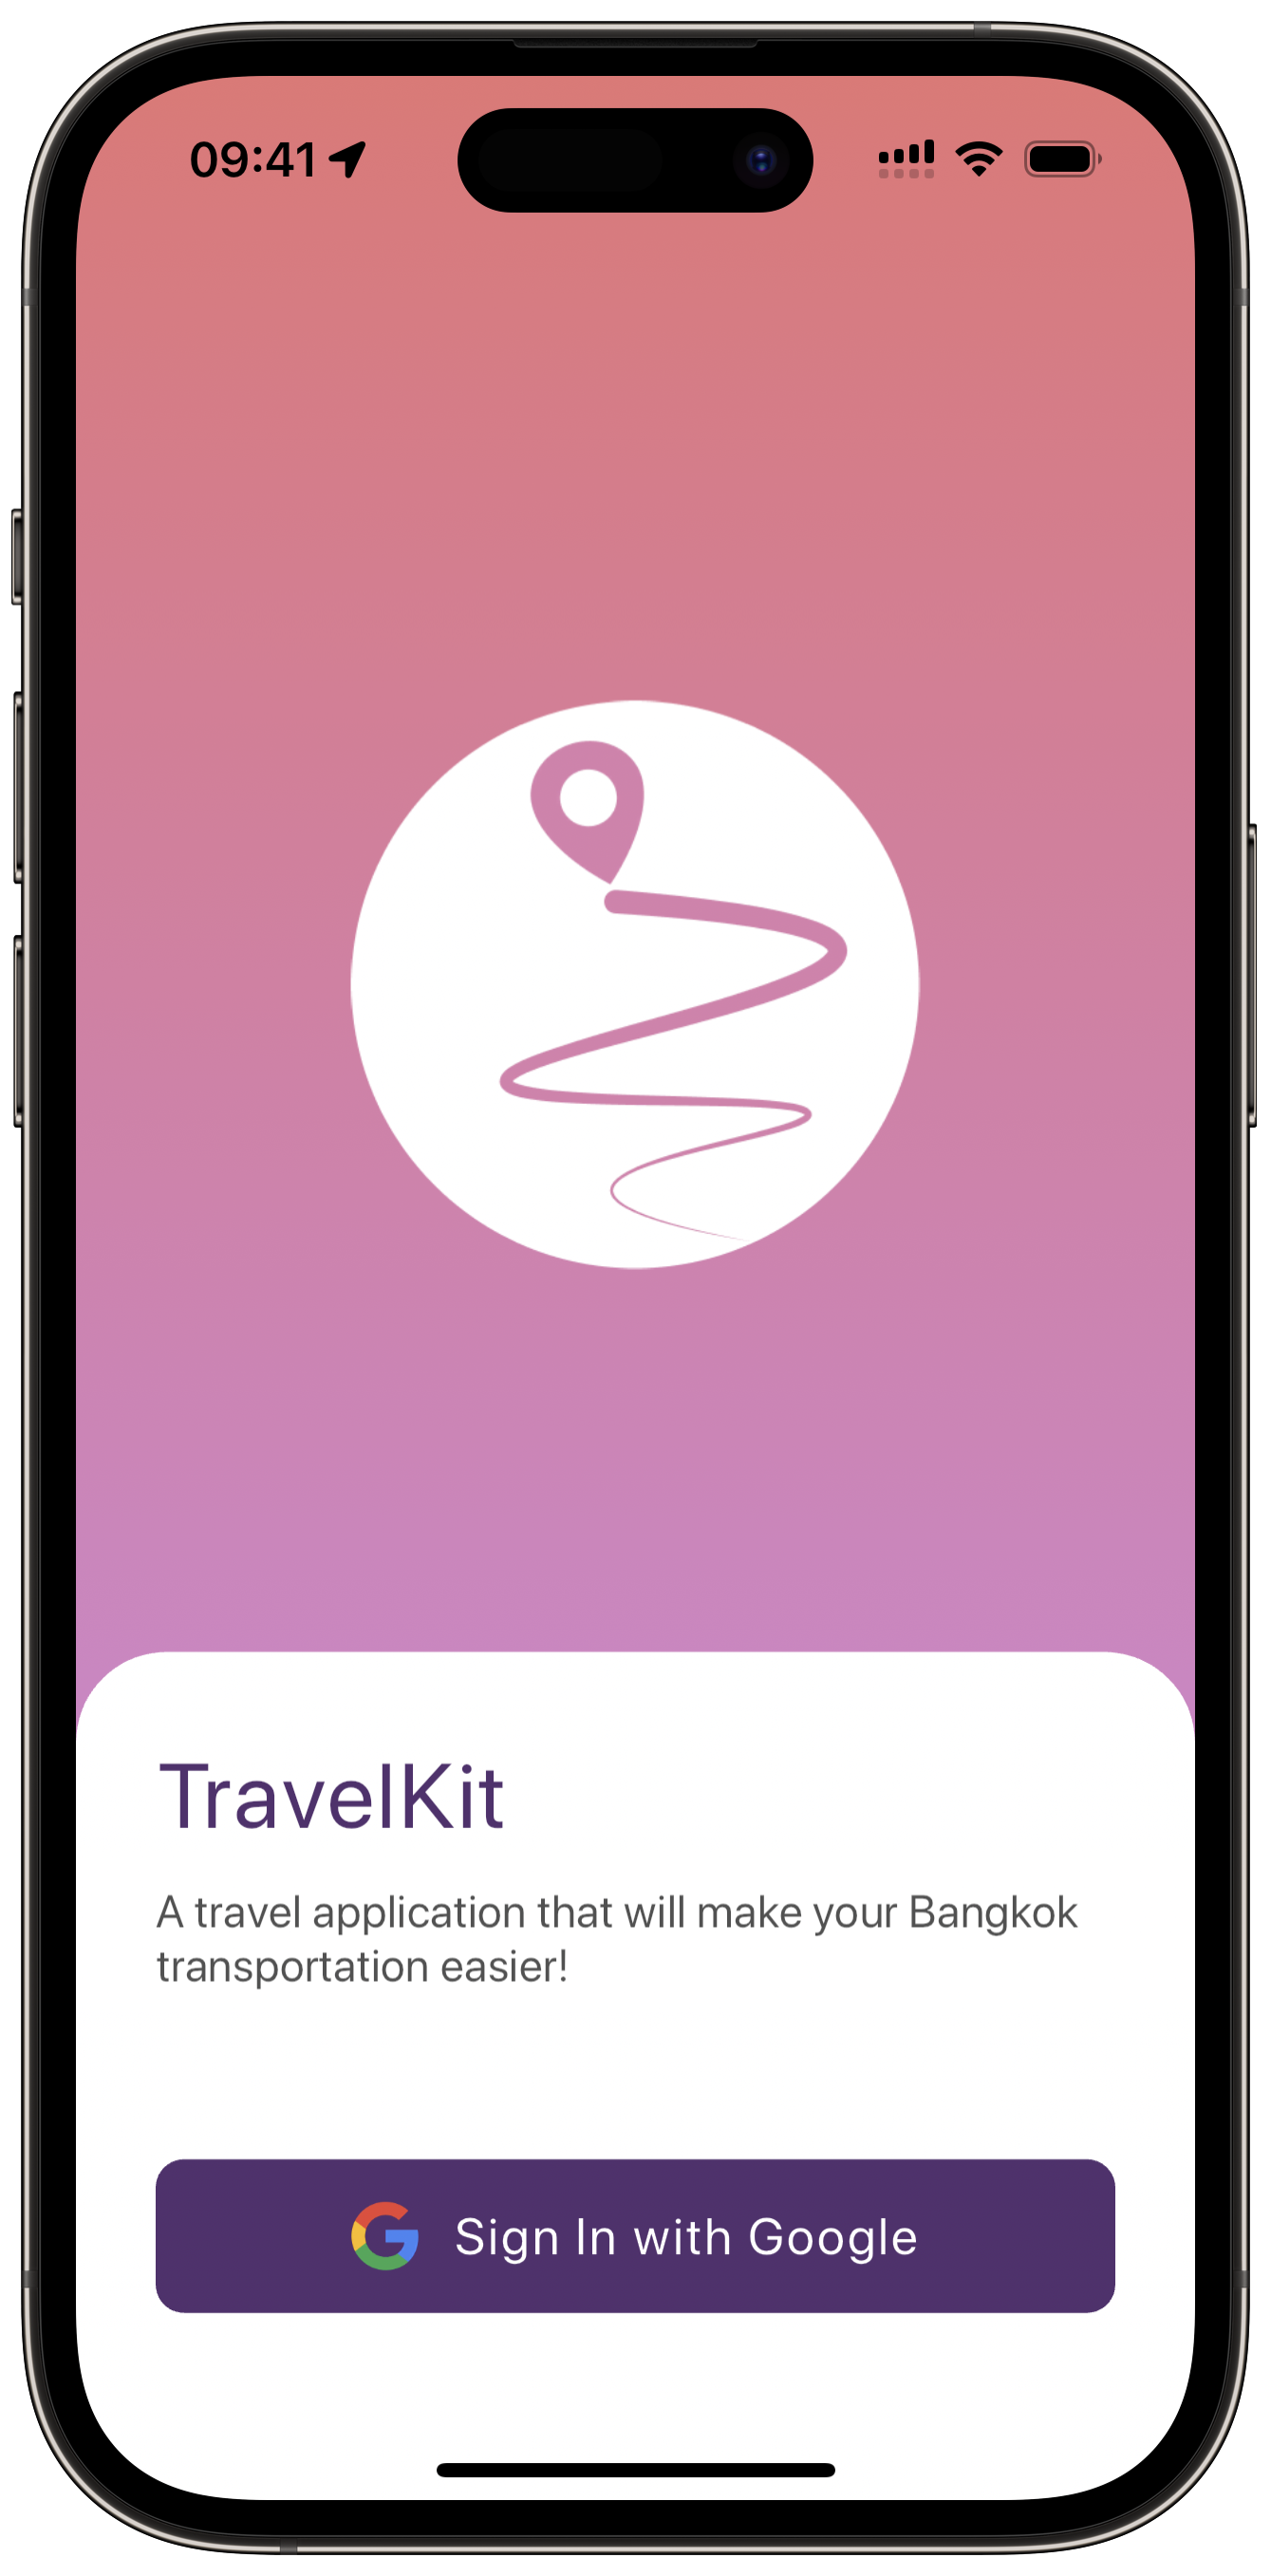
\includegraphics[width=0.5\linewidth]{chapter4/welcome_screen.png}
	\caption{Welcome screen}
	\label{fig:Welcome screen}
\end{figure}
This figure shows the welcome message and login button, Users can log in by Google to register and log into our application.

\newpage
\begin{figure}[!h]
	\centering
	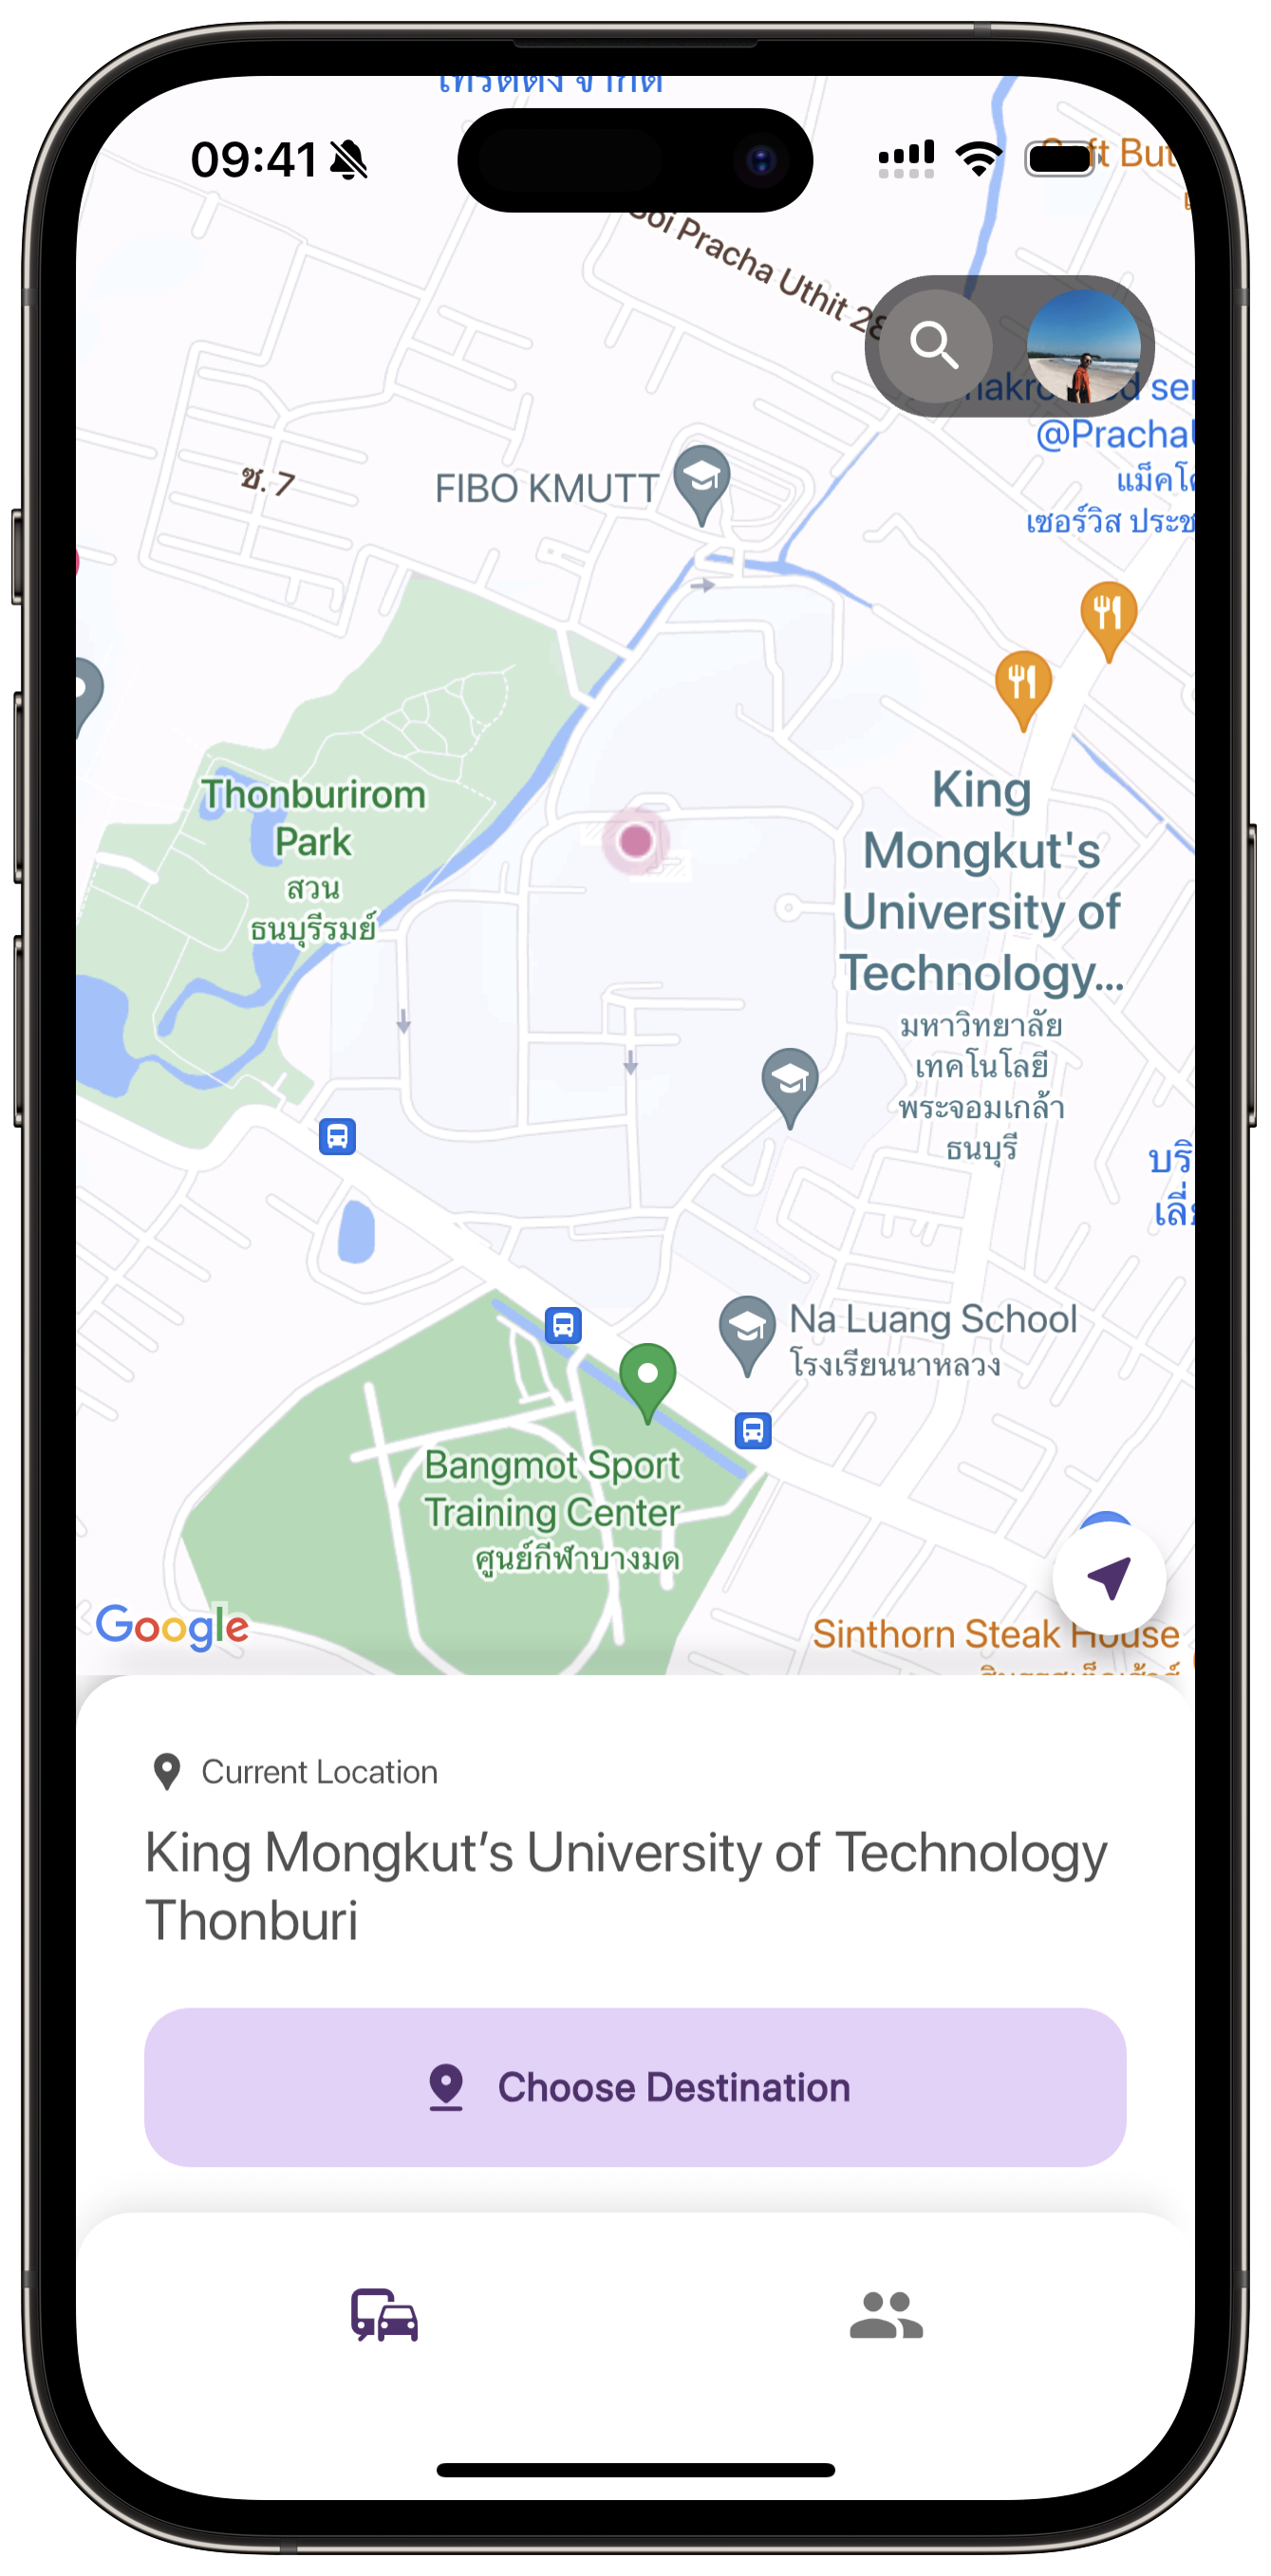
\includegraphics[width=0.5\linewidth]{chapter4/home_screen.png}
	\caption{Home screen}
	\label{fig:Home screen}
\end{figure}
This figure shows the map, current location, the name the current location after logging in and the user can tap the location icon to update the map screen to show their current location. The user can switch between the home screen and the community screen using the bottom navigation bar below.

\newpage
\begin{figure}[!h]
	\centering
	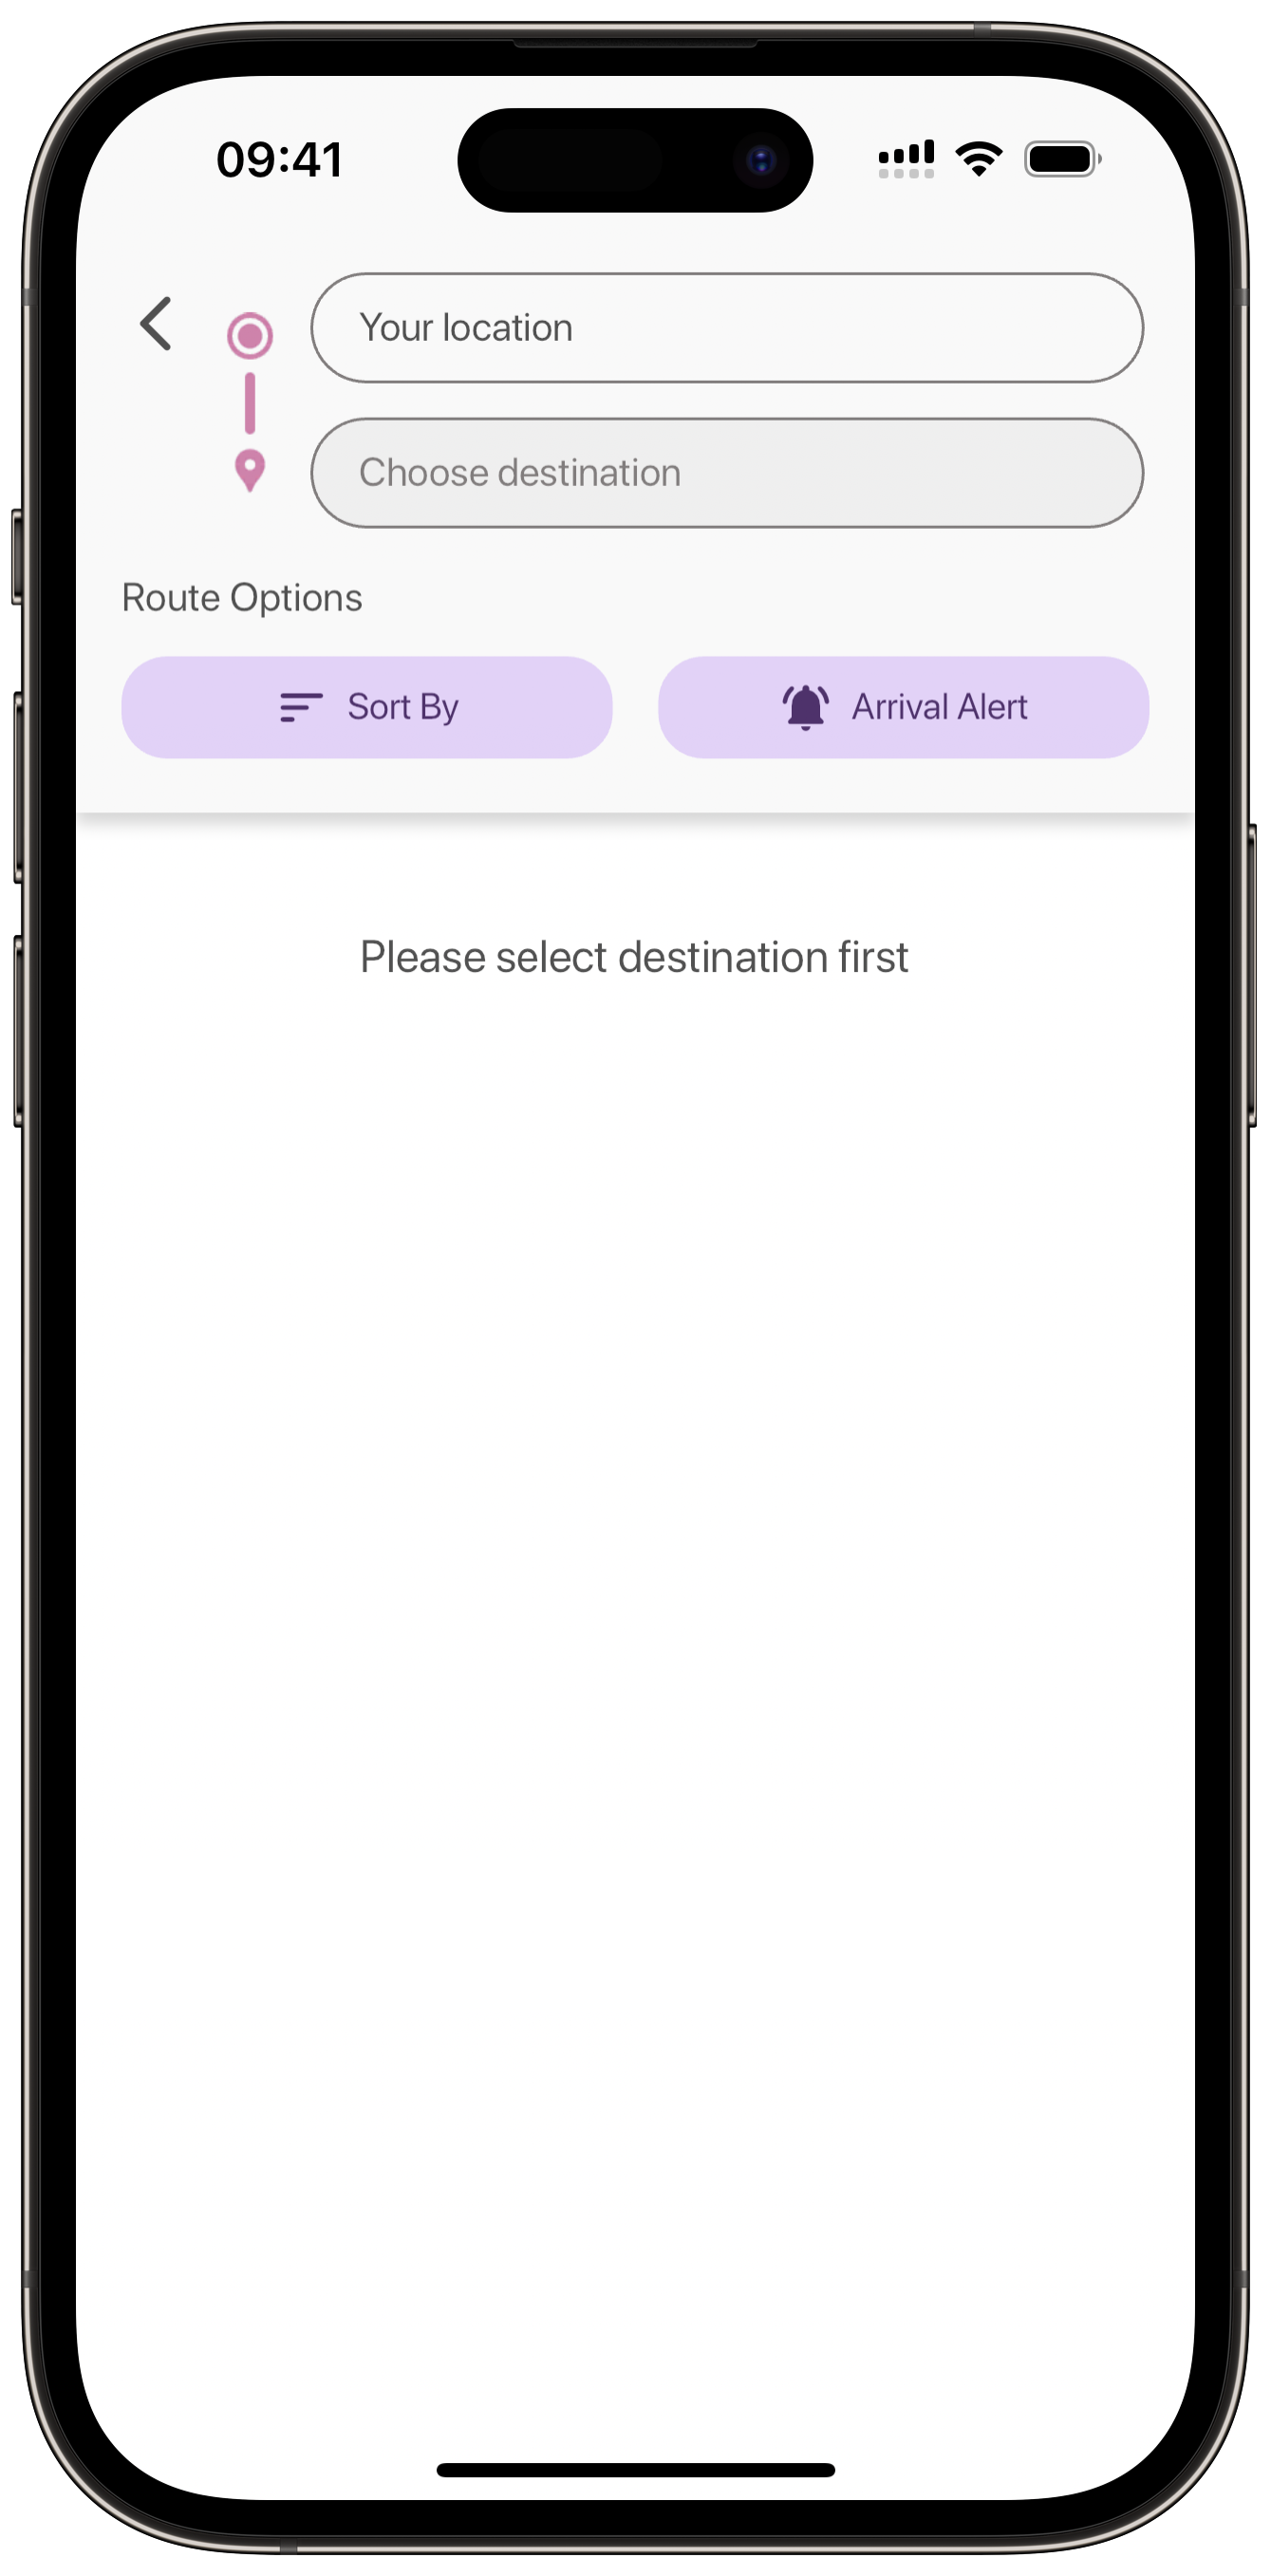
\includegraphics[width=0.5\linewidth]{chapter4/choosing_destination_screen.png}
	\caption{Choosing destination screen}
	\label{fig:Choosing destination screen}
\end{figure}
Users can search routes by specifying both the starting location and the destination to find routes for users.

\newpage
\begin{figure}[!h]
	\centering
	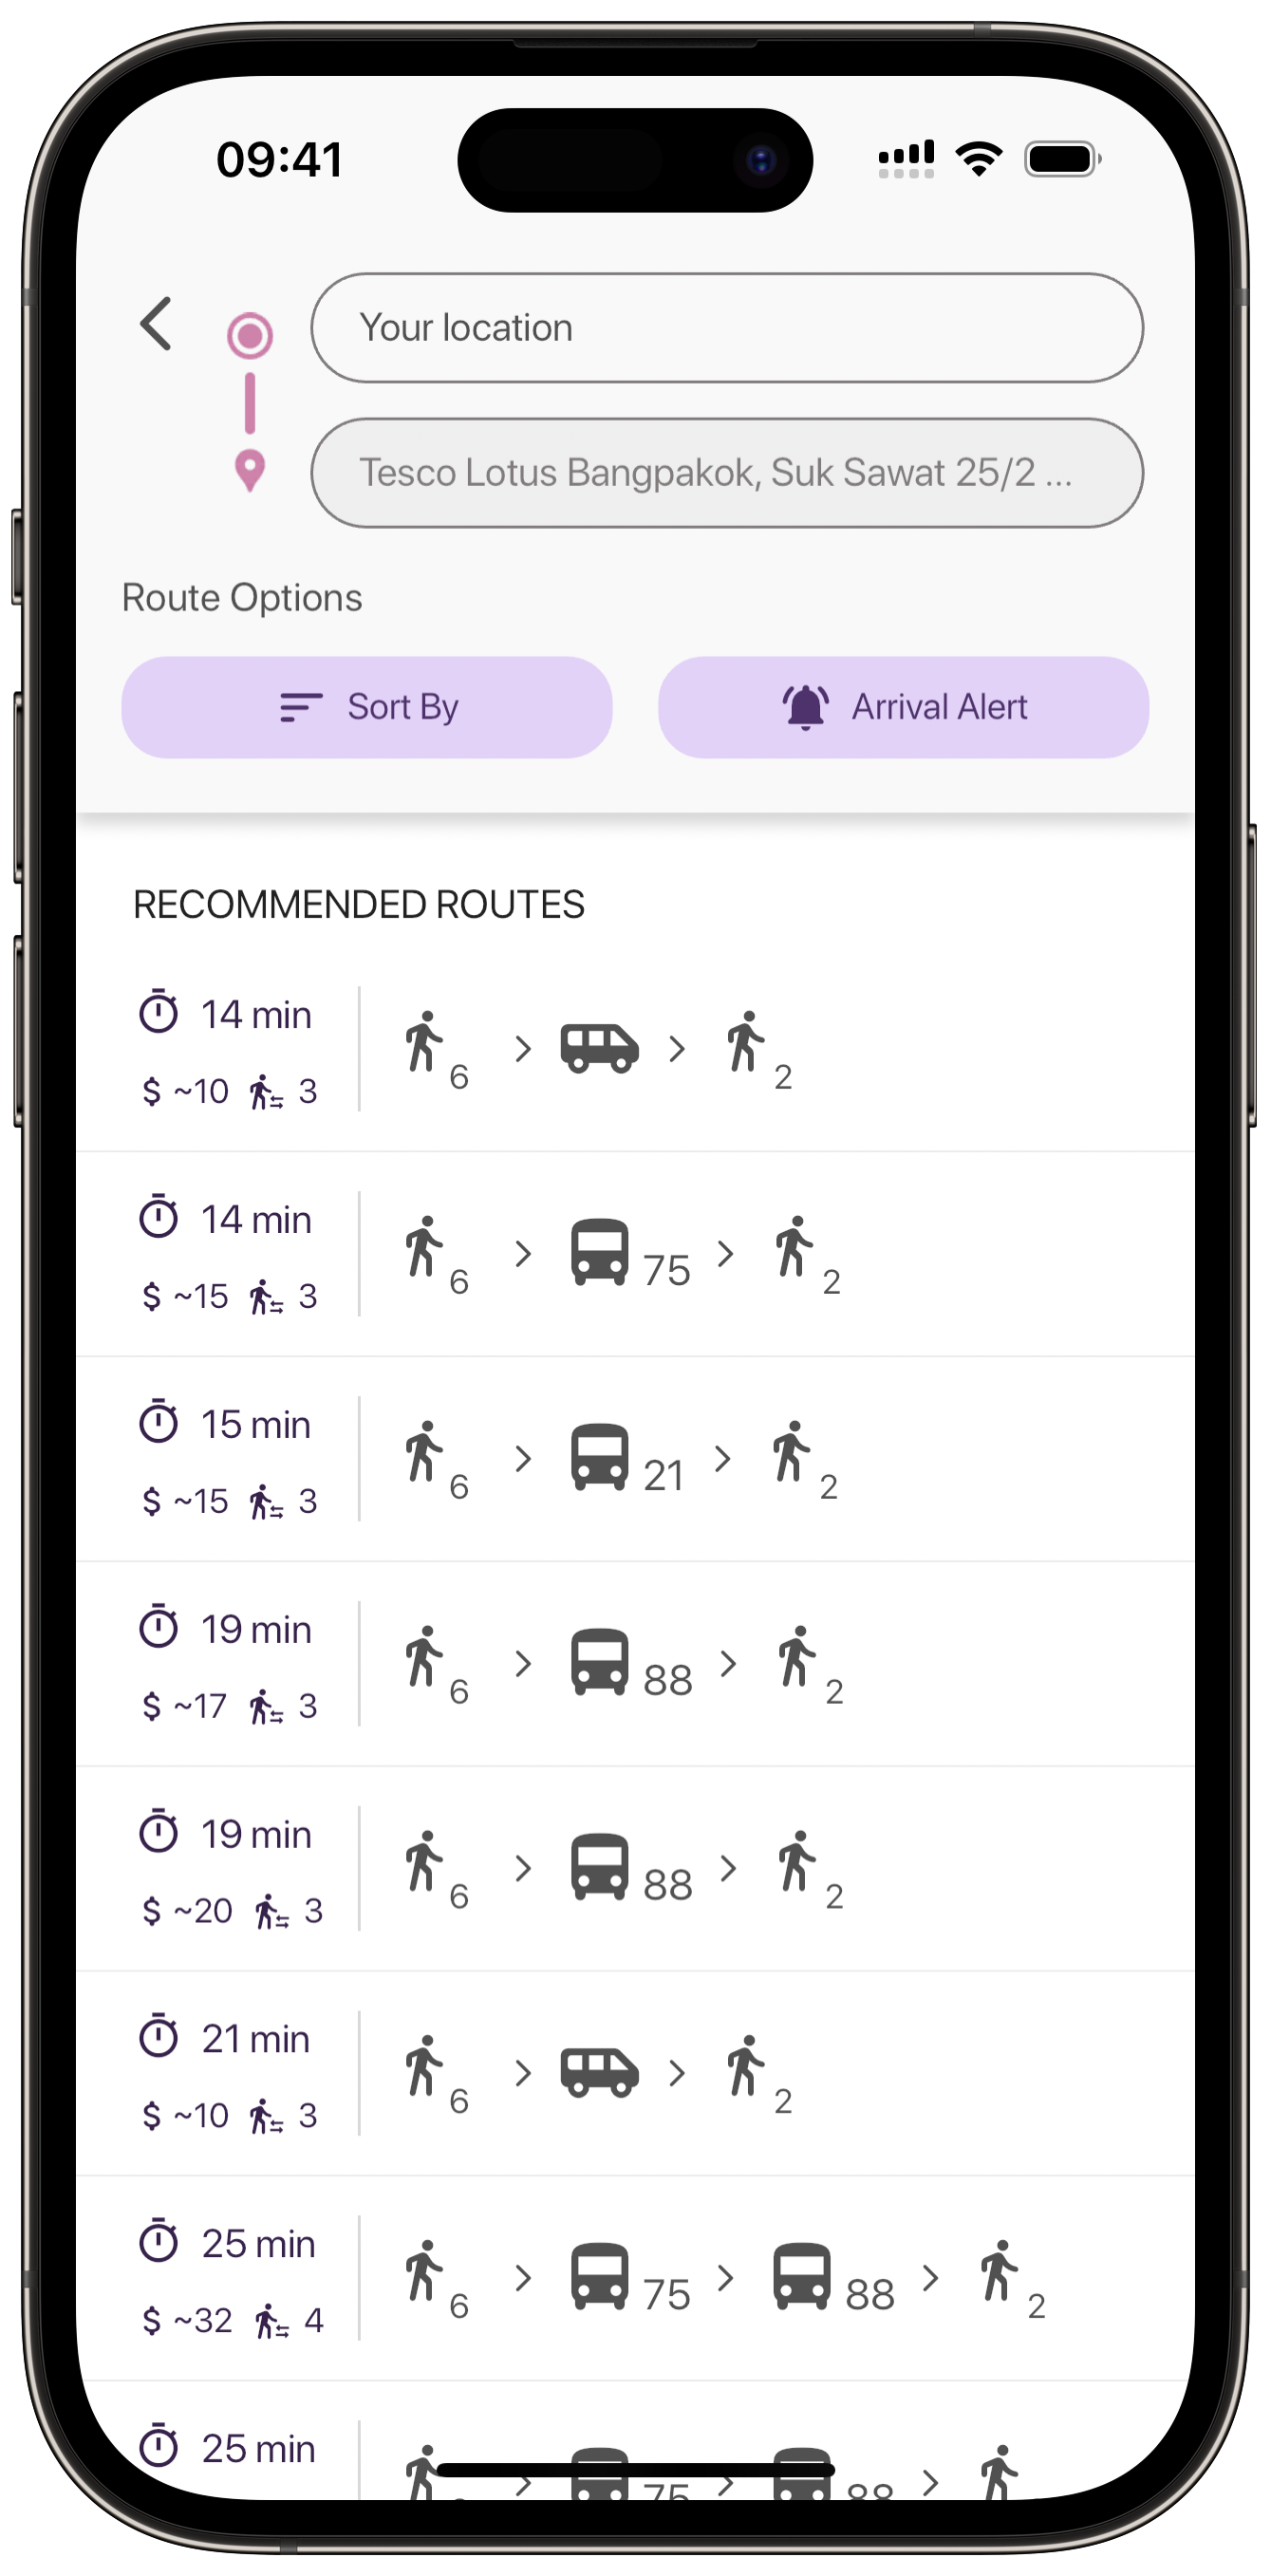
\includegraphics[width=0.5\linewidth]{chapter4/choosing_route_screen.png}
	\caption{Choosing route screen}
	\label{fig:Choosing route screen}
\end{figure}
This figure shows the search route results from the starting location to the destination. All routes are sorted by estimated time of arrival by default and users can see multiple routes to go to the destination.

\newpage
\begin{figure}[!h]
	\centering
	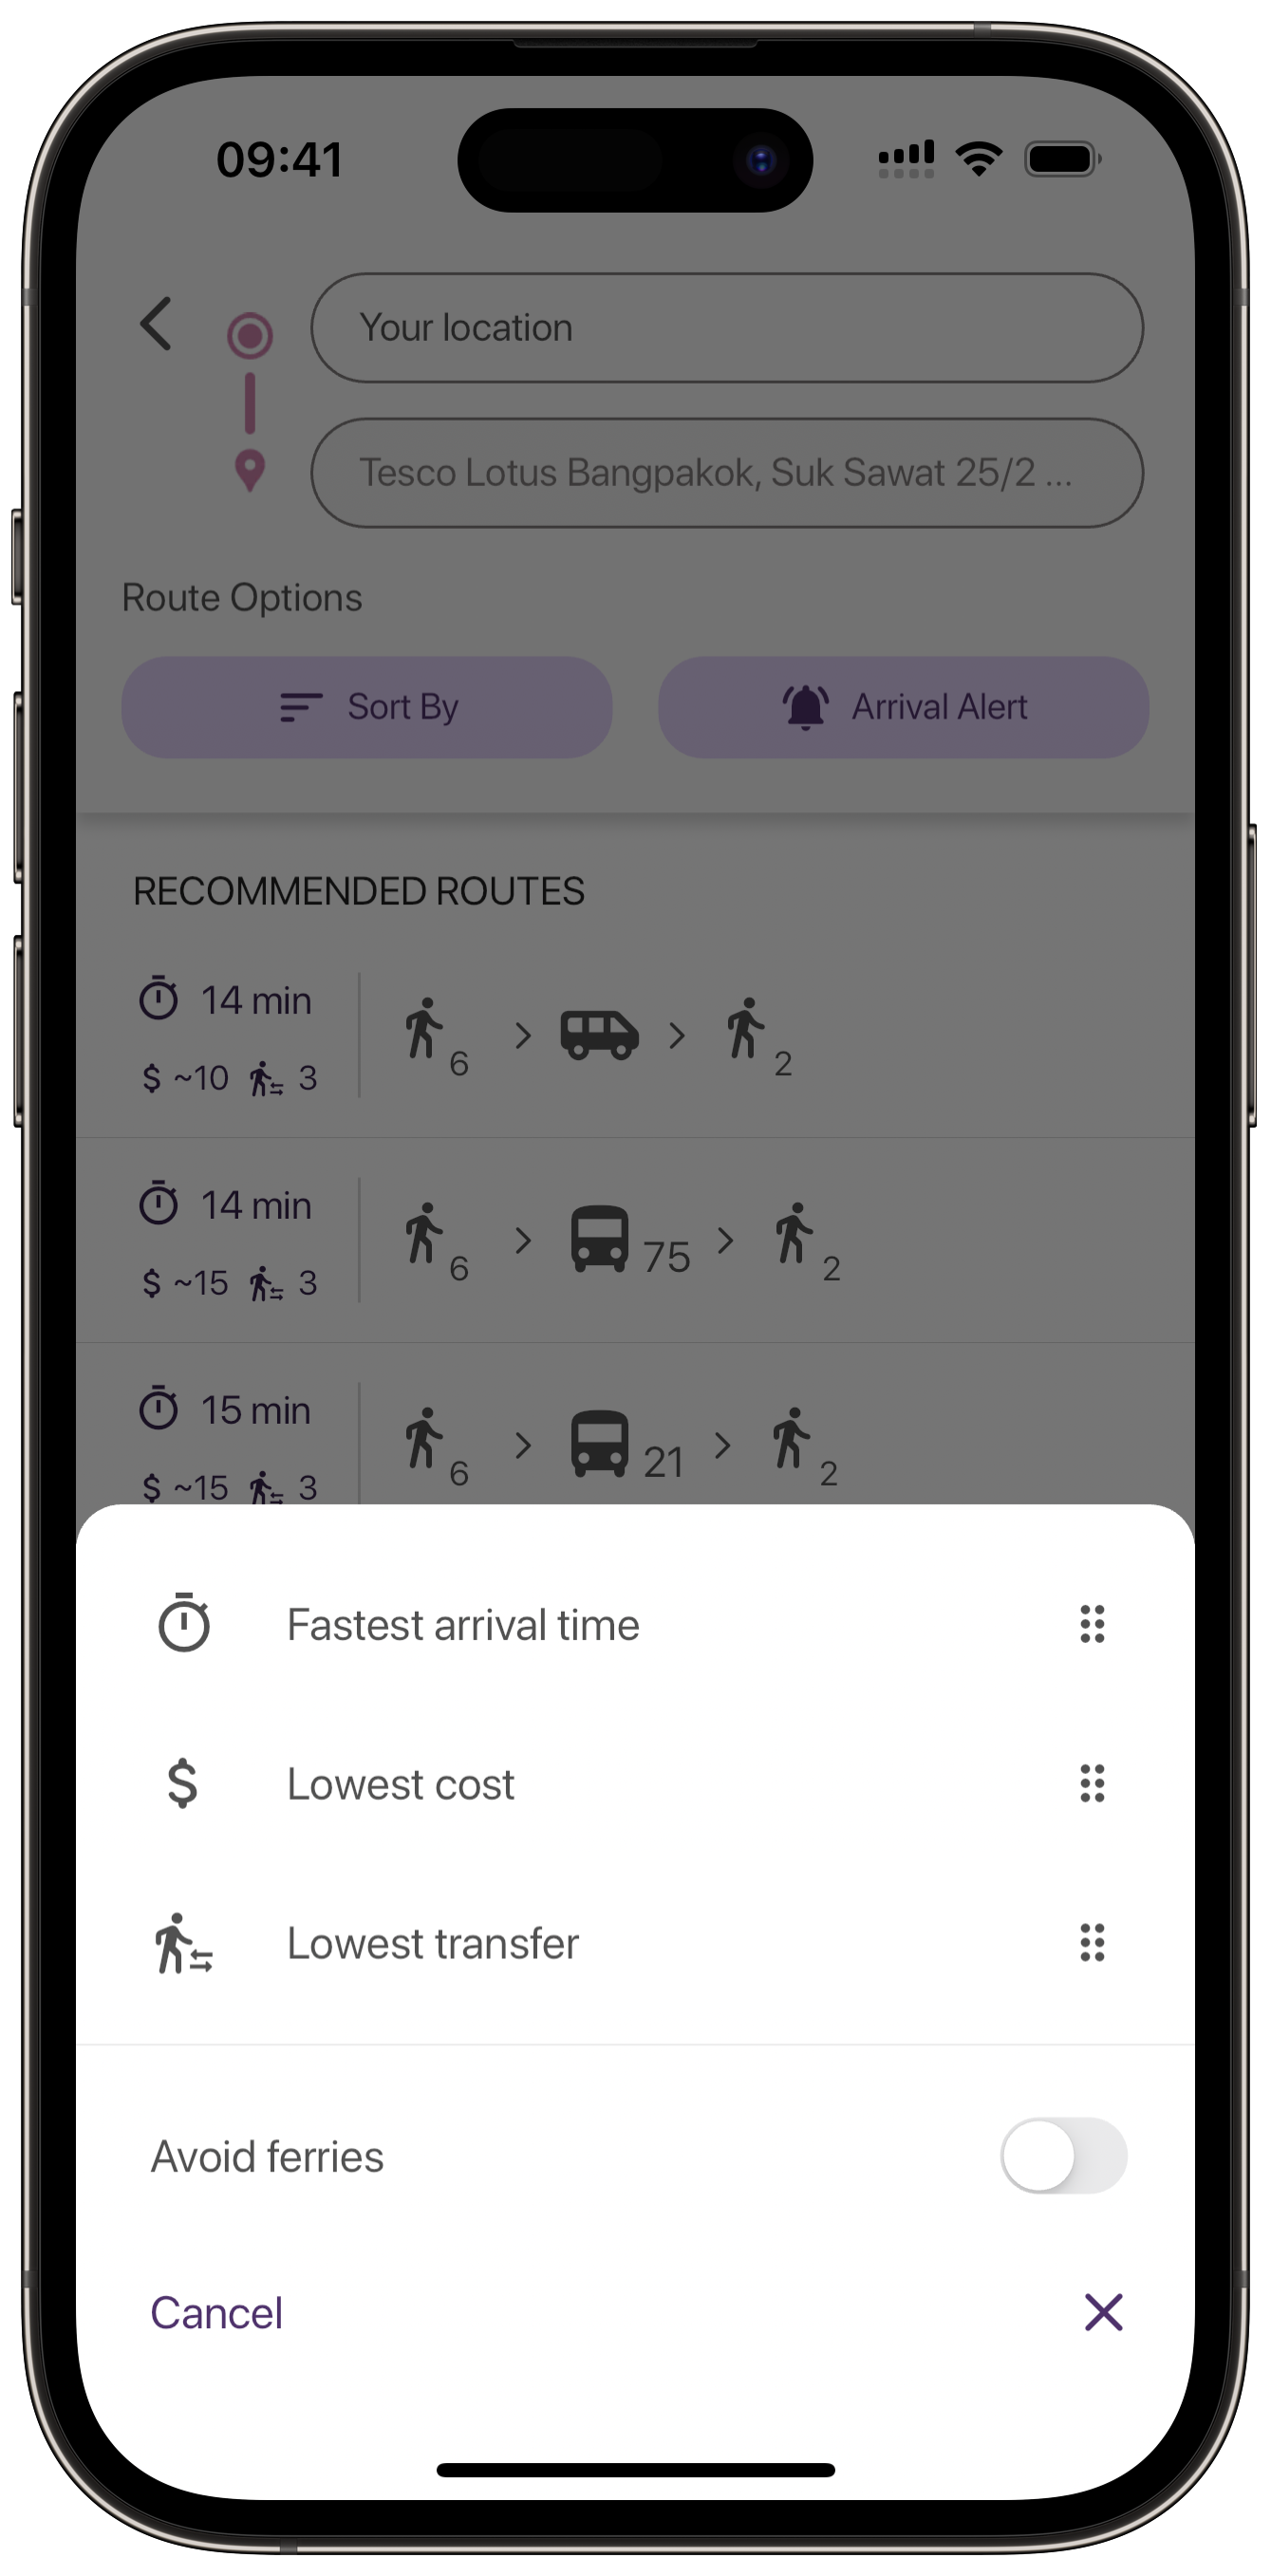
\includegraphics[width=0.5\linewidth]{chapter4/route_options_screen.png}
	\caption{Route options}
	\label{fig:Route options}
\end{figure}
The recommended routes can be sorted according to the user's preferences, such as the fastest arrival time, the cheapest price, the shortest transfer, and the avoid ferry option. 

\newpage
\begin{figure}[!h]
	\centering
	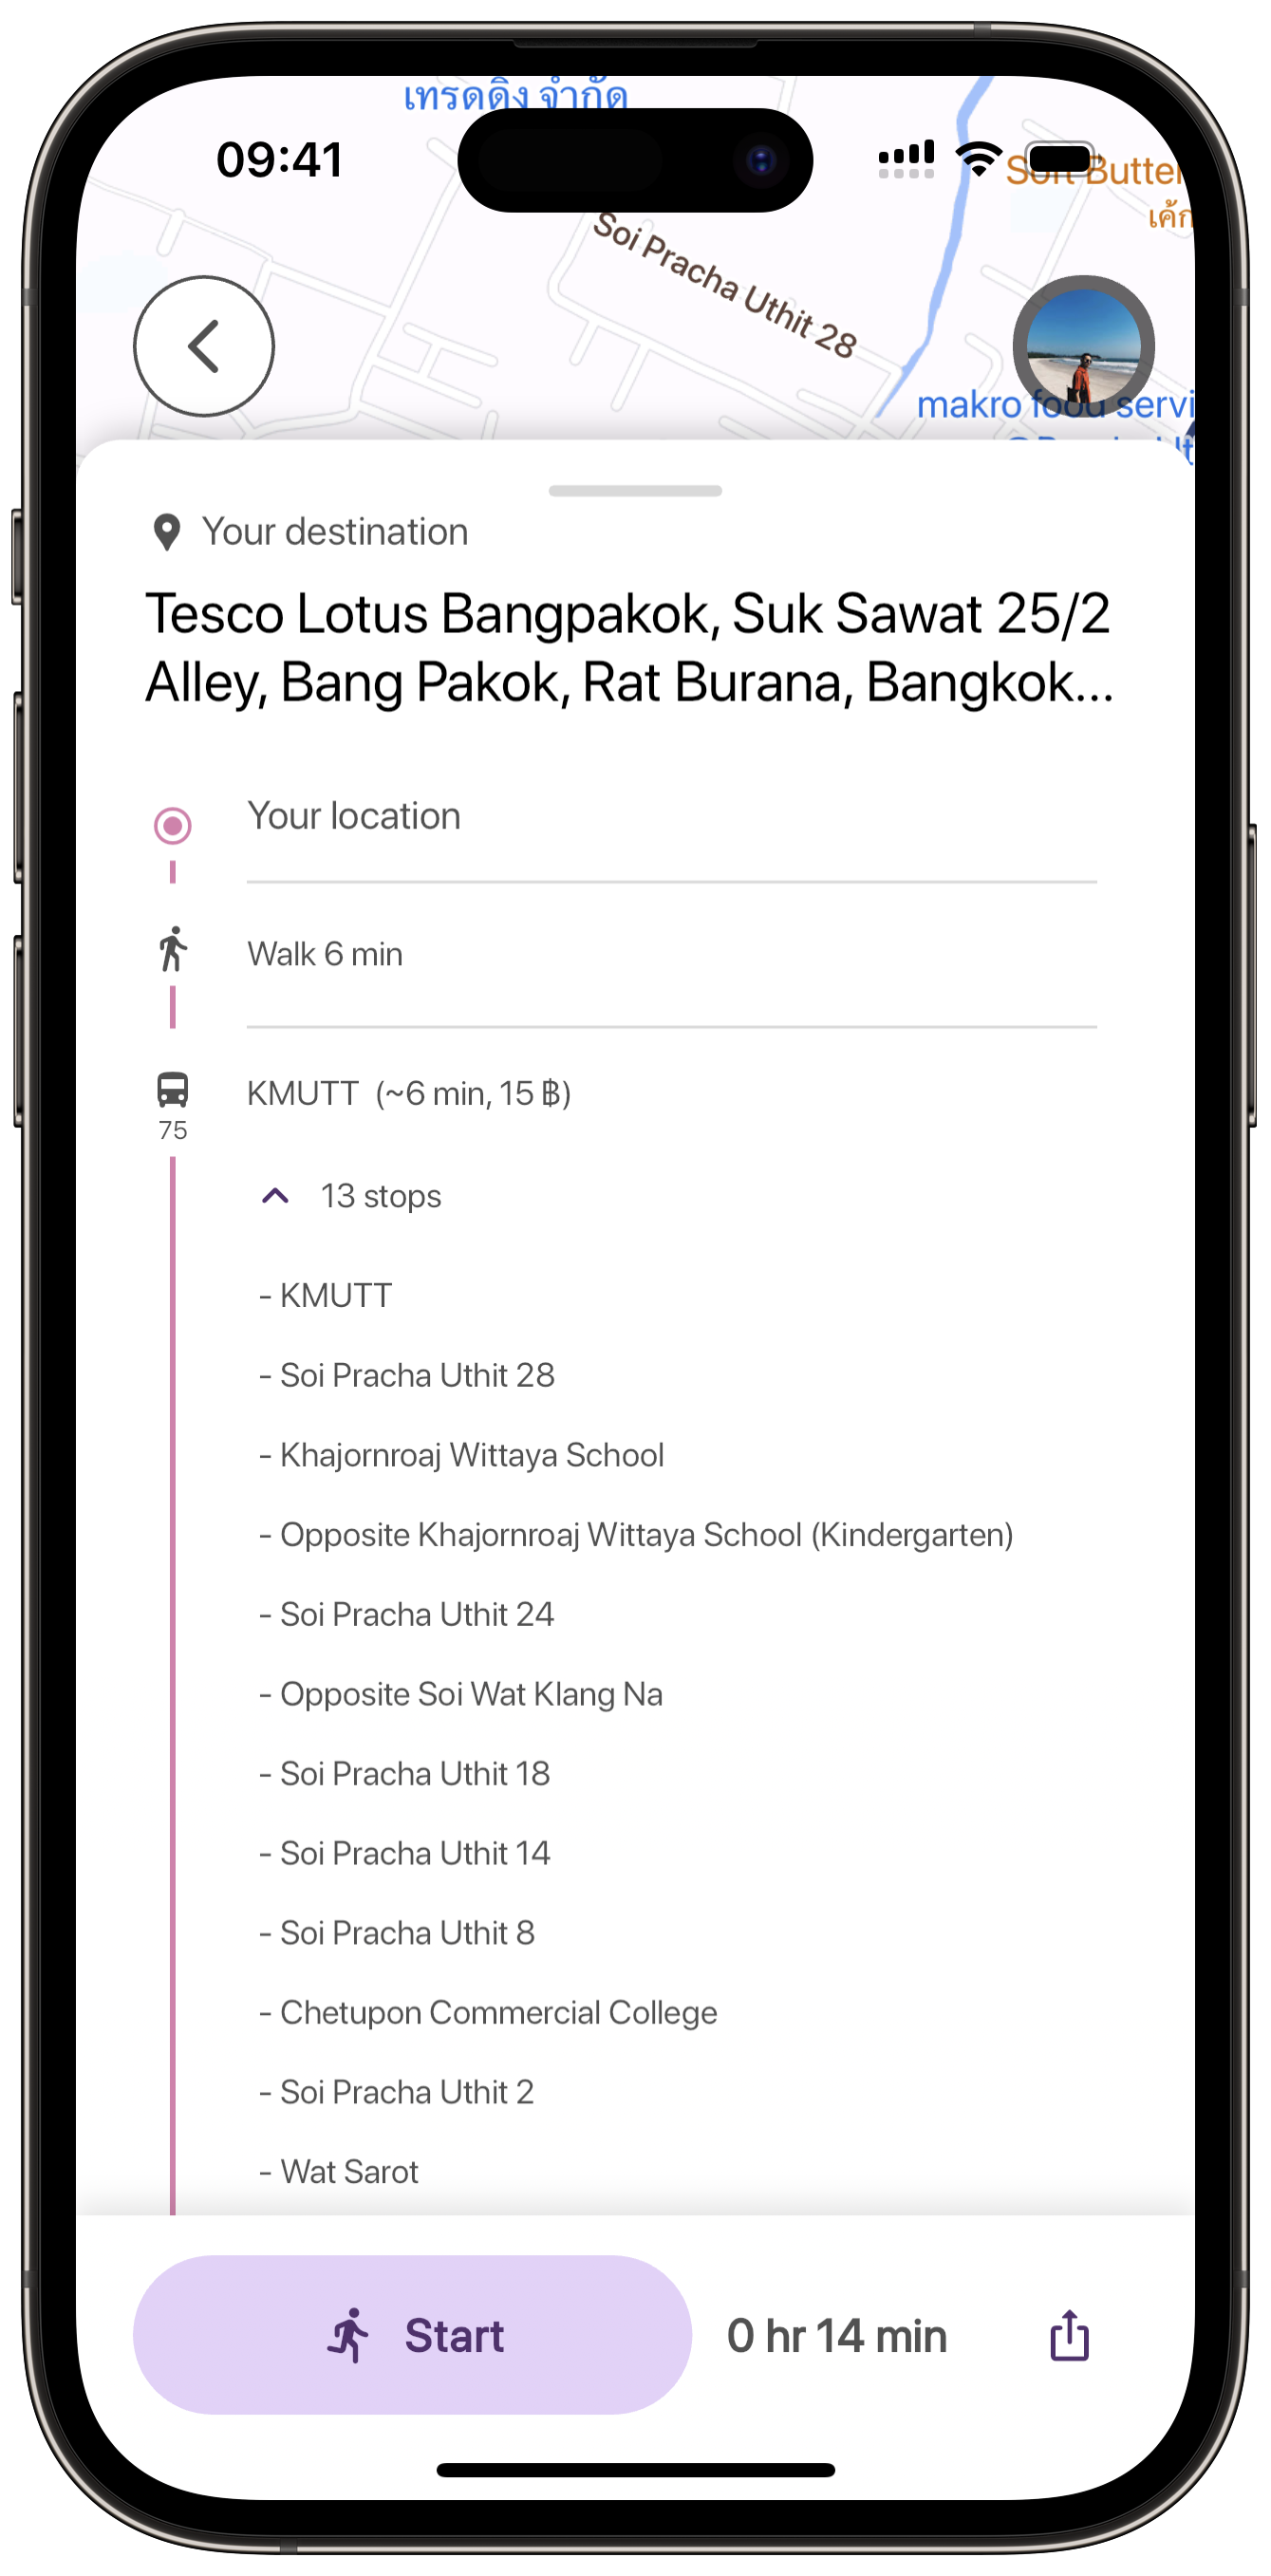
\includegraphics[width=0.5\linewidth]{chapter4/selected_route_detail_screen.png}
	\caption{Selected route detail screen}
	\label{fig:Selected route detail screen}
\end{figure}
After swiping up the bottom sheet, users will see the details of the selected route including cost, estimated time of arrival, and passed stop of each transport type. Users can tap the Start button for starting to real-time navigation or the Share icon to share the selected route with others.

\newpage
\begin{figure}[!h]
	\centering
	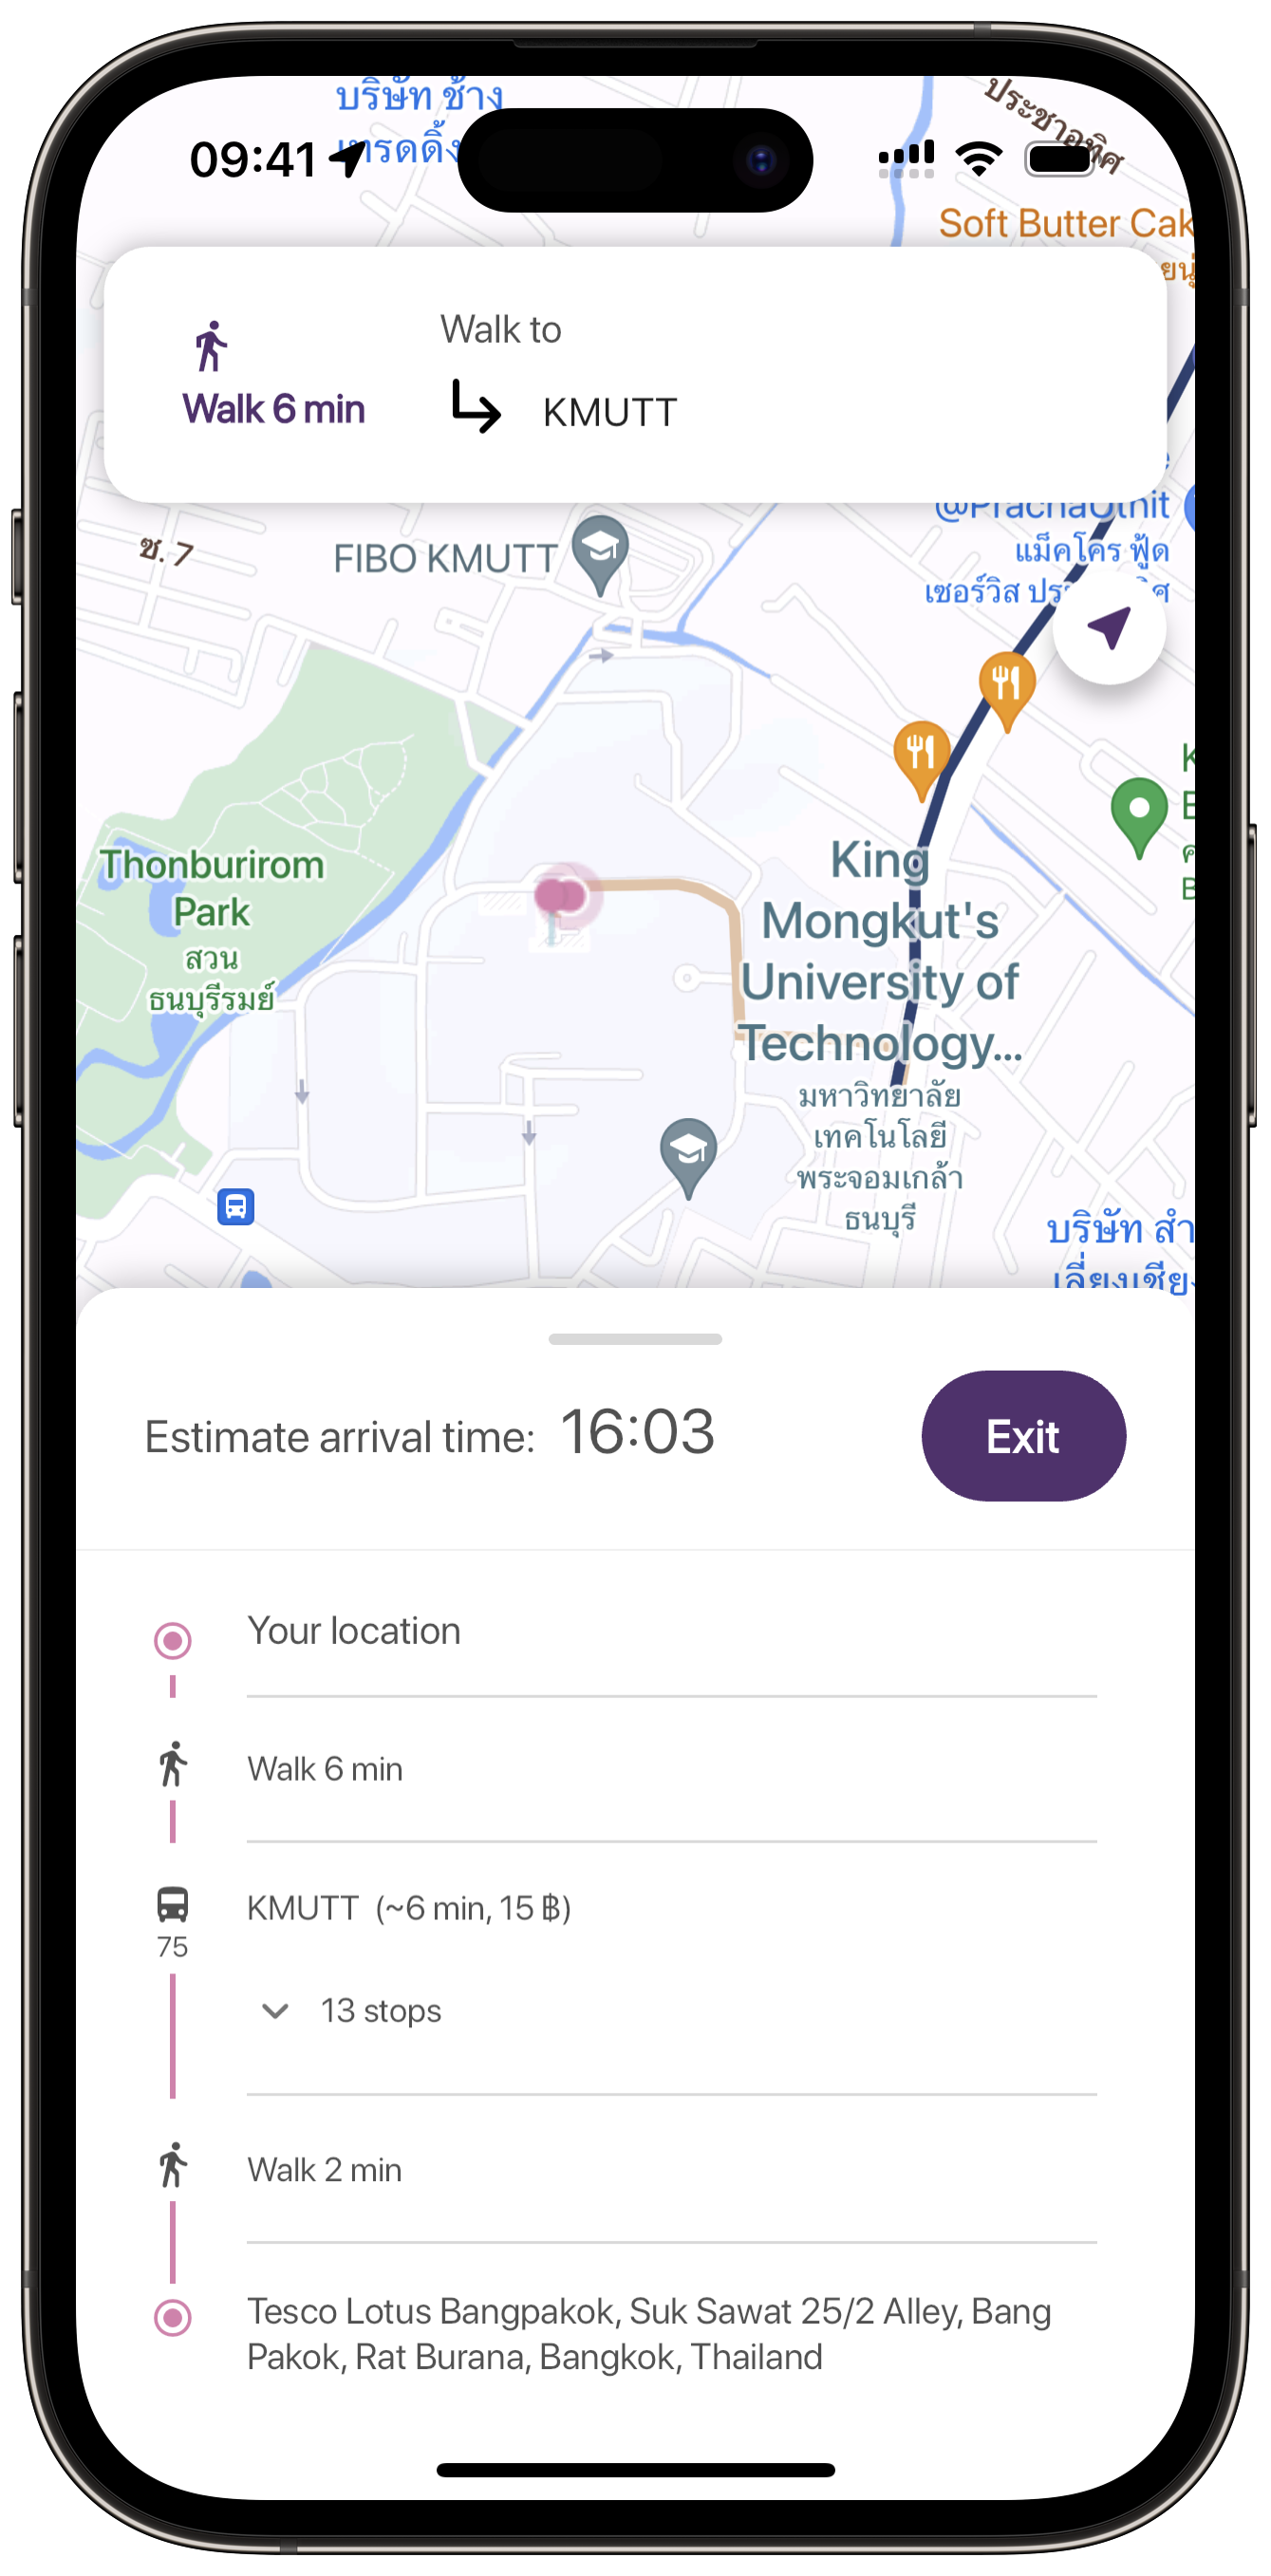
\includegraphics[width=0.5\linewidth]{chapter4/real_time_navigation_screen.png}
	\caption{Real-time navigation screen}
	\label{fig:Real-time navigation screen}
\end{figure}
This screen shows the details of the route in real-time including the current location, estimated arrival time, and the navigation overlay showing the current step with time and the next step at the top of the screen.

\newpage
\section{Test plan and test result}
\begin{table}[!h]
	\centering
	\resizebox{\linewidth}{!}{%
		\begin{tblr}{
				width = \linewidth,
				colspec = {Q[180]Q[350]Q[492]Q[100]},
				cell{3}{1} = {r=4}{},
				cell{7}{1} = {r=7}{},
				cell{14}{1} = {r=3}{},
				vlines,
				hline{1-3,7,14,17} = {-}{},
				hline{4-6,8-13,15-16} = {2-4}{},
			}
			Module         & Test expectation                                                   & Expected result                                                                                                  & Result  \\
			Authentication & Login with Google                                                  & Successful login to the system with user information provided                                                     & Success \\
			Home page      & Able to navigate between home page and community page              & Can change tab between two page                                                                                  & Success \\
			& Able to see the map with the current user location                  & See the map and correct current location                                                                         & Success \\
			& Able to logout from profile                                        & User is logged out                                                                                               & Success \\
			& Able to navigate to search page/ choose destination                & Navigate to search page correctly                                                                                & Success \\
			Routing        & Able to search for places                                          & User sees the list of places from Google API                                                                      & Success \\
			& Able to sort the route options                                     & User can change the sort by choices to change the travel preferences based on time, cost, and number of transfer & Success \\
			& Able to see the suggested routes when entering start and end location & User sees the list of suggested routes correctly with the details                                                 & Success \\
			& Able to navigate to see each route detail                          & User sees the route detail on the map and modal with travel time and cost                                         & Success \\
			& Able to share the route                                            & User gets a 6-digit code for sharing the route with other users                                                        & Success \\
			& Able to start the trip                                             & User navigates to the routing screen with a map and directions provided                                               & Success \\
			& Able to receive notification when an event happens                     & The system alerts the correct notification                                                                            & Success \\
			Community      & Able to get the exact route when searching by code                    & User navigates to the route detail page correctly                                                                     & Success \\
			& Able to see the suggested places                                   & List of suggested places displays correctly when entering the community page                                             & Success \\
			& Able to navigate to suggested routes page from suggested places    & User navigates to the routes selection page correctly                                                                 & Success 
		\end{tblr}
	}
	\caption{Table 4-1. Test Plan}
	\label{Table 4-1. Test Plan}
\end{table}
